\section{Materials and Methods}

\subsection{Datasets}

We evaluated five genotoxicity datasets (Table~\ref{tab:datasets}): three primary endpoints---Ames bacterial reverse mutation ($n = 13{,}560$), in~vitro chromosome aberration ($n = 1{,}619$), and in~vivo micronucleus ($n = 2{,}153$)---and two negative-sampled variants ($n = 345$ and $n = 231$) treated as exploratory supplementary analyses.

The Ames dataset combines pharmaceutical (drug-like) and industrial chemical sources. Compounds carry a source label based on their originating dataset; we use the term ``source'' to emphasize that this label reflects data provenance---encompassing potential differences in chemical space, data quality, and labeling conventions---rather than a computed chemical classification. Drug-sourced compounds ($n = 6{,}416$) had a positive rate of 58.3\%, while industrial-sourced compounds ($n = 7{,}144$) had 3.0\%, a 19.5-fold difference. The in~vitro and in~vivo datasets lacked source annotations. Label conflicts (compounds with contradictory labels across sources) were resolved by exclusion: 169 for Ames, 3 for in~vitro, and 2 for in~vivo.

Cross-endpoint overlap analysis revealed substantial compound sharing: 97.5\% of in~vitro and 92.1\% of in~vivo compounds also appear in Ames, with moderate label concordance (Cohen's $\kappa = 0.14$--$0.20$). The three endpoints largely probe the same chemical universe through different biological readouts.

All datasets were split 80/20 into training and test partitions using scaffold-based splitting\cite{Sheridan_2013} with zero scaffold-group overlap. Murcko scaffolds\cite{Bemis_Murcko_1996} were generated with RDKit;\cite{RDKit} acyclic compounds were clustered by agglomerative clustering on Morgan fingerprint\cite{Rogers_Hahn_2010} similarity.

\begin{table}[ht]
\caption{Dataset summary. Positive rate refers to the training partition. The 375 total configurations comprise 5 datasets $\times$ 3 preprocessing scenarios $\times$ (6 tabular models $\times$ 4 feature modes + 1 GNN).}
\label{tab:datasets}
\centering
\small
\begin{tabular}{@{}llrrrrr@{}}
\toprule
Dataset & Assay & $n$ & Train & Test & Pos.\ rate (\%) & Scaffolds \\
\midrule
Ames & Bacterial reverse mutation & 13,560 & 10,848 & 2,712 & 29.1 & 1,691 \\
In vitro CA & Chromosome aberration & 1,619 & 1,295 & 324 & 10.4 & 353 \\
In vivo MN & Micronucleus & 2,153 & 1,722 & 431 & 3.7 / 2.8\textsuperscript{a} & 410 \\
\midrule
In vitro CA (sampled)\textsuperscript{b} & Neg.\ sampled CA & 345 & 276 & 69 & 49.6 & 169 \\
In vivo MN (sampled)\textsuperscript{b} & Neg.\ sampled MN & 231 & 184 & 47 & 33.3 & 129 \\
\bottomrule
\end{tabular}

\medskip
\footnotesize
\textsuperscript{a}Training / test positive rate.
\textsuperscript{b}Supplementary exploratory datasets.
\end{table}

\subsection{Preprocessing Scenarios}

Each dataset was processed under three scenarios: \textbf{raw} (original SMILES), \textbf{salt-stripped} (largest fragment retained via RDKit's \texttt{LargestFragmentChooser},\cite{RDKit} followed by charge normalization---modifying 45\% of Ames, 81\% of in~vitro, and 83\% of in~vivo SMILES), and \textbf{no-metal} (compounds containing metal atoms excluded).

\subsection{Feature Representations}

Five representations were evaluated. \textbf{Compact} (138 features) combined 13 physicochemical descriptors (MW, LogP, TPSA, HBD, HBA, rotatable bonds, fraction $\mathrm{C_{sp3}}$, aromatic ring count, ring count, heteroatom count, heavy atom count, formal charge, valence electrons) with 125 structural alerts based on Benigni--Bossa SA1--SA31,\cite{Benigni_Bossa_2008,Benigni_2013} Kazius toxicophores,\cite{Kazius_2005} and ISS Ames alerts. \textbf{Broad FP-512/1024/2048} (266/394/522 features) extended compact with 128/256/384 Morgan fingerprint bits\cite{Rogers_Hahn_2010} selected by mutual information\cite{Kraskov_2004} on the training set only (bits with prevalence below 1\% or above 99\% were excluded). \textbf{Graph} representations used molecular graphs with 9-dimensional atom features and normalized adjacency matrices, paired exclusively with the GCN.

\subsection{Algorithms}

Seven classifiers were evaluated: XGBoost,\cite{Chen_XGBoost_2016} LightGBM,\cite{Ke_LightGBM_2017} Random Forest,\cite{Breiman_2001} SVM with RBF kernel,\cite{Cortes_Vapnik_1995} Logistic Regression,\cite{Cox_1958} a 128--64 MLP with early stopping,\cite{Rumelhart_1986} and a three-layer Graph Convolutional Network\cite{Kipf_Welling_2017} with LayerNorm and global mean pooling. SVM and Logistic Regression used standard scaling. Class imbalance was addressed via \texttt{scale\_pos\_weight} or \texttt{class\_weight='balanced'}. Hyperparameter tuning used \texttt{RandomizedSearchCV} with \texttt{GroupKFold} (scaffold groups).\cite{Pedregosa_sklearn_2011}

\subsection{Three-Level Evaluation Framework}

For fair comparison across evaluation methods, we defined a single locked configuration---XGBoost, compact features, raw SMILES---and applied it at three levels (Figure~\ref{fig:framework}):

\textbf{Level 1 (in-domain test):} the scaffold-split held-out test set, with bootstrap 95\% CIs (500 iterations) on MCC,\cite{Matthews_1975} ROC-AUC, PR-AUC, balanced accuracy, sensitivity, specificity, and Brier score.\cite{Brier_1950}

\textbf{Level 2 (split-method comparison):} 5-fold stratified random CV and 5-fold scaffold-grouped CV, both with 5 repeats, on the full dataset.

\textbf{Level 3 (cross-source LDO):} for Ames, trained on one source and tested on the other, using the locked configuration plus LightGBM and Random Forest to assess algorithm-specific robustness.

\subsection{Additional Analyses}

\textbf{Full grid:} all 375 configurations were evaluated on the scaffold-split test set ($5 \text{ datasets} \times 3 \text{ scenarios} \times [6 \text{ tabular} \times 4 \text{ feature modes} + 1 \text{ GNN}] = 375$).

\textbf{Applicability domain (AD):} Tanimoto similarity on 1024-bit Morgan fingerprints,\cite{Rogers_Hahn_2010} threshold $\geq 0.3$.

\textbf{Feature importance:} SHAP values\cite{Lundberg_SHAP_2017} (\texttt{TreeExplainer}) for tree-based models on the three primary endpoints.

\textbf{Learning curves:} 10\%--100\% training fractions with 5-fold scaffold CV, using the locked configuration only.

\textbf{Statistical comparison:} McNemar's test\cite{McNemar_1947} with continuity correction for the top two models per endpoint.

\textbf{Threshold tuning:} out-of-fold probability-based threshold optimization with 5-fold \texttt{GroupKFold}.

\textbf{LDO threshold decomposition:} to disentangle prior shift from genuine source shift, we computed LDO MCC at three thresholds: default ($t = 0.5$), prior-corrected ($t$ = training positive rate, optimal under pure prior shift), and oracle ($t$ maximizing MCC on the test set, an upper bound on threshold-based recalibration). The implementation is provided as \texttt{ldo\_threshold\_analysis.py} in the supplementary materials.

\begin{figure}[ht]
\centering
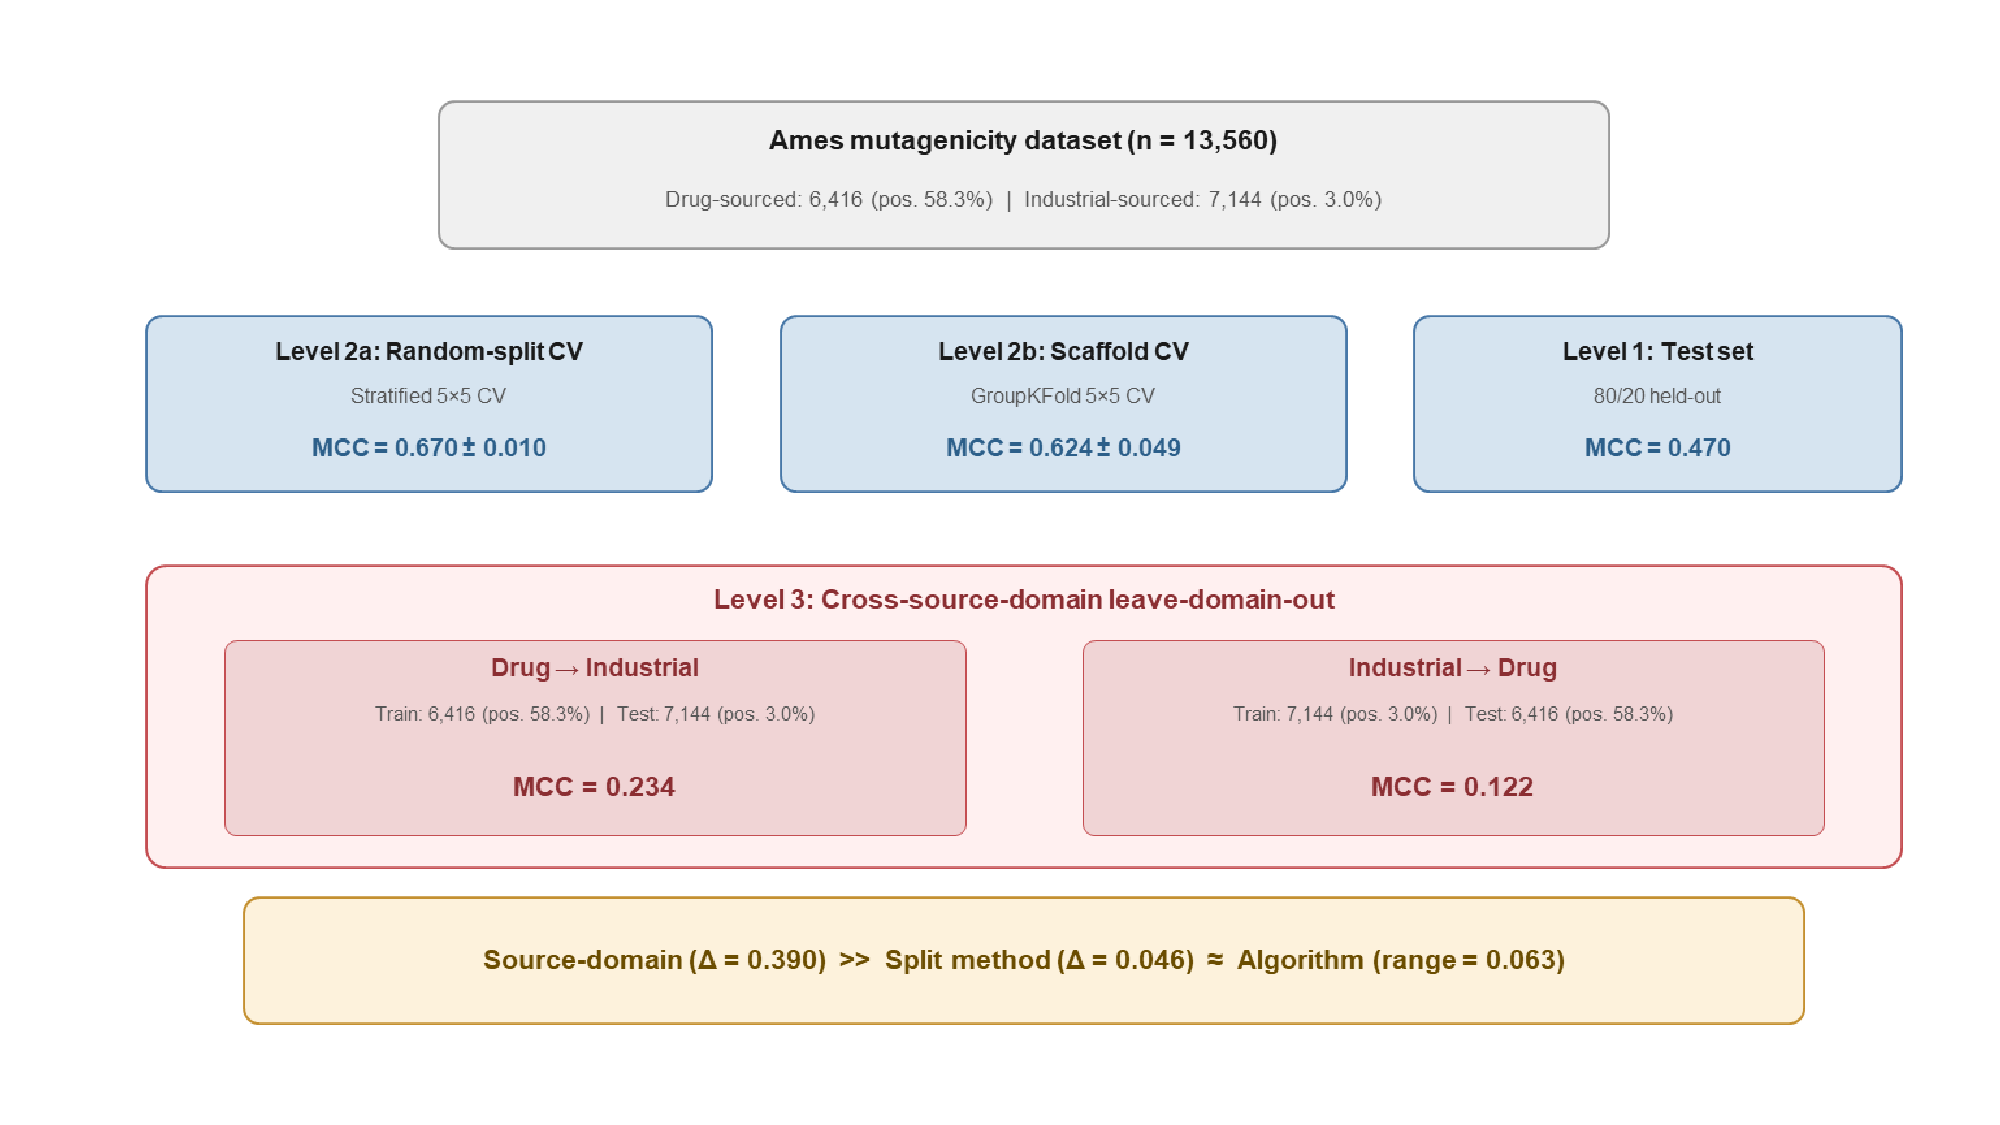
\includegraphics[width=\textwidth]{figures/figure1_framework.pdf}
\caption{Three-level evaluation framework. All levels use the same locked configuration (XGBoost, compact features, raw SMILES), enabling fair MCC comparison across evaluation methods. The overestimation hierarchy summarizes the relative magnitudes observed in this benchmark.}
\label{fig:framework}
\end{figure}
